\documentclass[twocolumn,superscriptaddress, prb]{revtex4-1}
\setlength{\parskip}{0mm }
\setlength{\belowcaptionskip}{-10pt}
\usepackage{amsfonts}
\usepackage{amssymb}
\usepackage{amsmath}
\usepackage{amsthm}
\usepackage{dsfont}
\usepackage[dvipdfm]{graphicx}
\usepackage{stackrel}
\usepackage{color}

% Should come last b/c it needs to overload a bunch of commands
\usepackage{hyperref}

\newcommand{\ket}[1]{|#1\rangle}
\newcommand{\bra}[1]{\langle #1 |}



\begin{document}
\title{Unsuspected conserved quantities in a nonintegrable quantum system}

\author{Hyungwon Kim}
\affiliation{Physics Department, Princeton University, Princeton, NJ 08544, USA}
%\affiliation{Max-Planck-Institut f$ {\ddot{u}}$r Quantenoptik, Hans-Kopfermann-Str. 1, 85748 Garching, Germany}

\author{Mari Carmen Ba${\rm{\tilde n}}$uls}
\affiliation{Max-Planck-Institut f$ {\ddot{u}}$r Quantenoptik, Hans-Kopfermann-Str. 1, 85748 Garching, Germany}

\author{J. Ignacio Cirac}
\affiliation{Max-Planck-Institut f$ {\ddot{u}}$r Quantenoptik, Hans-Kopfermann-Str. 1, 85748 Garching, Germany}

\author{Matthew B. Hastings}
\affiliation{Station Q, Microsoft Research, Santa Barbara, CA 93106-6105, USA}
\affiliation{Quantum Architectures and Computation Group, Microsoft Research, Redmond, WA 98052, USA}

\author{David A. Huse}
\affiliation{Physics Department, Princeton University, Princeton, NJ 08544, USA}

\begin{abstract}
Modified.
We numerically construct slowly thermalizing local operators in one-dimensional chain of spin-1/2 with a nonintegrable Hamiltonian.
Restricting the support of operators to $M$, we exhaustively search for the operator that minimizes the Frobenius norm of the commutator
with the Hamiltonian and thus changes slowly.  We find that operators are present with significantly slower relaxation than would be
expected from a hydrodynamic description.  Similar slowly relaxing operators are found for a Floquet system and for quantum circuits, in both cases where no local conservation law is present.  We argue that such slow relaxation may be a generic feature of local systems, showing the existence of unsuspected conserved quantities.
\end{abstract}

\pacs{}

\maketitle

%\section{Introduction}
It has been proposed that an isolated quantum system can still thermalize, in the sense that local observables approach their value in thermal  equilibrium\cite{Deutsch:1991,Srednicki:1994,Rigol:2008}.  The presence of conserved quantities such as spin leads to relaxation to a generalized ensemble.  Experimental studies have increased the interest in this question\cite{Polkovnikov:2011, Yukalov:2011}.  One proposed theoretical explanation is the eigenstate thermalization hypothesis (ETH)\cite{Deutsch:1991,Srednicki:1994,Rigol:2008,Santos:2010,Rigol:2012,Kruczenski:2013,Beugeling:2014,Sorg:2014,Kim_ETH}, which argues that many-body eigenstates of non-integrable Hamiltonians have local density matrices that are thermal; then, at late times, decoherence between different energy eigenstates produces a thermal density matrix.

However, not all systems show this local thermalization in an accessible time scale\cite{Banuls:2011}.
One possibility is that the ETH is false for the system of Ref.~\onlinecite{Banuls:2011}; another possibility is that the time scales required to thermalize locally are too long to be numerically accessible.  The question is: how can such a slow time scale arise, when a non-integrable system like the one studied has no conserved local quantities other than energy?

In this work, we show how such a large time scale can emerge by showing that indeed conserved (or, more precisely, approximately conserved) quantities {\it are} present in many non-integrable systems.  We construct these operators numerically, by explicitly searching for operators with a small commutator with the Hamiltonian.  One source of such operators with a small commutator are those that result from local fluctuations in the energy density.  However, we show numerically, that these are {\it not} the operators with the smallest commutator.  Instead, other operators are present with a much smaller commutator, presenting ``unsuspected conserved quantities" for these systems.  For numerical reasons discussed below, much of our work focuses on the Frobenius norm rather than operator norm to measure relaxation, but we also discuss the operator norm.


The time scale of energy relaxation is discussed below, where we construct operators describing local energy fluctuation in a subinterval.  This time scale matches the expectation
 from hydrodynamics:
$D k^2$, where $D$ is diffusivity and the momentum $k$ is inversely proportional to the interval length.
However, numerically we find that the time scale for the slowest operator that we constructed diverges as a {\it faster} power of length than the decay of the operators associated with energy fluctuations, and for the observed system sizes, the time scale is quantitatively larger.

To further understand the presence of such approximately conserved quantities we then turn to a Floquet system where energy is not a local conserved quantity.
Nevertheless, we observe some slowly relaxating operators in the Floquet system.
To test this, we also consider several random unitaries constructed from local quantum circuits, and in every case we again find slowly relaxing operators.
In fact, we argue that such slow relaxing operators must be present in any Floquet system or in any quantum circuit.  However, these slowly relaxing operators are in a sense morally similar to the slowly relaxing operator in a Hamiltonian system describing energy fluctuations: these operators are present in any such system, so long as locality is present.  They themselves do not inhibit relaxation of the local density matrices ``as fast as possible" (i.e., on a time scale proportional to the length of the interval; see Ref.~\onlinecite{Brandao:2012} for a proof that this happens for random local circuits).  Thus, the real surprise is our numerical observation that there are other operators in some Hamiltonian systems with even slower relaxation.

%\section{Model and Method}
%\subsection{Model}
%\subsection{Method}

As a nonintegrable model Hamiltonian, we choose a semi-infinite spin-1/2 Ising chain with both longitudinal and transverse fields.
\footnote{We have also performed similar analysis in the infinite chain with translation invariance. Most of our main results (figure \ref{fig:full_optimal})
remains true. Since translation non-invariant system is easier to visualize the local operators and to directly compare with diffusive energy mode, here we present the results on the semi-infinite chain.}
\begin{align}
H = \sum_{i=1}^{\infty} g\sigma^x_i + h\sigma^z_i + \sigma^z_i \sigma^z_{i+1} ~,
\label{eq:Hamiltonian}
\end{align}
where $\sigma^x_i$ and $\sigma^z_i$ are Pauli matrices of the spin at site $i$.
Ref.~\onlinecite{Banuls:2011} has found a nonthermalizing state for this model within the accessible time scale.
We choose $(g,h) = (0.905, 0.809)$, at which this model is known to be robustly nonintegrable even for a relatively small system size \cite{Kim:2013}
that can be explored by exact diagonalization method \footnote{see Supplementary material for another choice of parameters}

We consider local operators supported on a finite interval; an operator supported on sites $i=1$ to $i=M$ is said to have ``range $M$".
Each traceless operator
$\hat{A}_M$ can always be expressed by a linear combination of $4^M - 1$ traceless basis operators (excluding the identity).
Therefore, we write
\begin{align}
\hat{A}_M = \sum_{\ell = 1}^{4^M - 1} c_\ell \hat{O}_{M,\ell} ~,
\end{align}
where $c_\ell$ is a real number ($\hat{A}_M$ should be hermitian) and $\hat{O}_{M,\ell}$ is the corresponding basis operator.
We choose $\hat{O}_{M,\ell}$ to be mutually orthogonal using the Hilbert-Schmidt inner product so that
$\mathrm{tr(\hat{O}_{M,\ell} \hat{O}_{M,k})} = 0$ for $\ell\neq k$.

The time derivative of an operator is proportional to its commutator with the Hamiltonian.
Therefore, we want to {\it minimize} the magnitude of $[\hat{A}_M, H]$
to construct a slowly relaxing local operator of length $M$.
Using the square of the Frobenius norm, $\mathrm{tr(\hat{O}\hat{O}^\dag)}$, to measure this magnitude\footnote{There are three widely used norms of an operator;
the operator norm (largest absolute value of the operator), the trace norm ($\mathrm{tr(\sqrt{\hat{O}\hat{O}^\dag})}$),
and the Frobenius norm ($\sqrt{\mathrm{tr(\hat{O}\hat{O}^\dag)}}$). Each norm has its own meaning.
Although the operator norm is physically the most relevant one for our purpose,
we choose the Frobenius norm since it is the easiest to numerically optimize.
See supplementary material for details of the relevance of the operator norm.},
we wish to minimize:
\begin{align}\label{eq:minimize}
\frac{\mathrm{tr([\hat{A}_M,H][\hat{A}_M,H]^\dag)}}{\mathrm{tr(\hat{A}_M\hat{A}^\dag_M)}} = \sum_{\ell,k}\frac{c_\ell c_k \mathrm{tr([\hat{O}_{M,\ell},H][\hat{O}_{M,k},H]^\dag)}}{\sum_j c_j ^2 \mathrm{tr((\hat{O}_{M,j})^2)}} ~.
\end{align}
This is a standard quadratic optimization problem.
Since the Hamiltonian has time-reversal symmetry,
we can consider even and odd operators under time-reversal separately.
It turns out that for $M\geq 4$, $\hat{A}_M$ that minimizes Eq. \eqref{eq:minimize} always comes from the even sector.

First, let's understand what this quantity means.
We consider an initial mixed state $\rho$ such as
\begin{align}\label{eq:initial}
\rho = \frac{1}{Z}\left(I + \epsilon \hat{A}_M\right) ~,
\end{align}
where $Z$ is the normalization factor, $I$ is the identity, and $\epsilon$ is a small positive number.
$\hat{A}_M$ serves as a small inhomogeneity in the infinite temperature ensemble.
Now we look at how $\hat{A}_M$ decays as a function of time:
$\langle \hat{A}_M(t) \rangle = \mathrm{tr(\rho e^{iHt} \hat{A}_M e^{-iHt})} = (\epsilon/Z)\mathrm{tr(\hat{A}_M e^{iHt} \hat{A}_M e^{-iHt})}$.
In other words, we look at the two-point correlation of $\hat{A}_M$ in the time domain with the infinite temperature background.
Trivially, the first order time derivative at $t = 0$ is zero. The second order time derivative at $t = 0$ is
\begin{align}
\frac{d^2}{dt^2}\langle \hat{A}_M(t)\rangle\bigg|_{t=0} = \frac{\epsilon}{Z}\mathrm{tr([\hat{A}_M,H][\hat{A}_M,H]^\dag)} ~.
\end{align}
Therefore,by minimizing Eq. \eqref{eq:minimize},
we search for the slowest relaxing operator at early time.
Although we instead want a slowly relaxing operator at long time,
this minimization already gives nontrivial results as we report below.


\begin{figure}
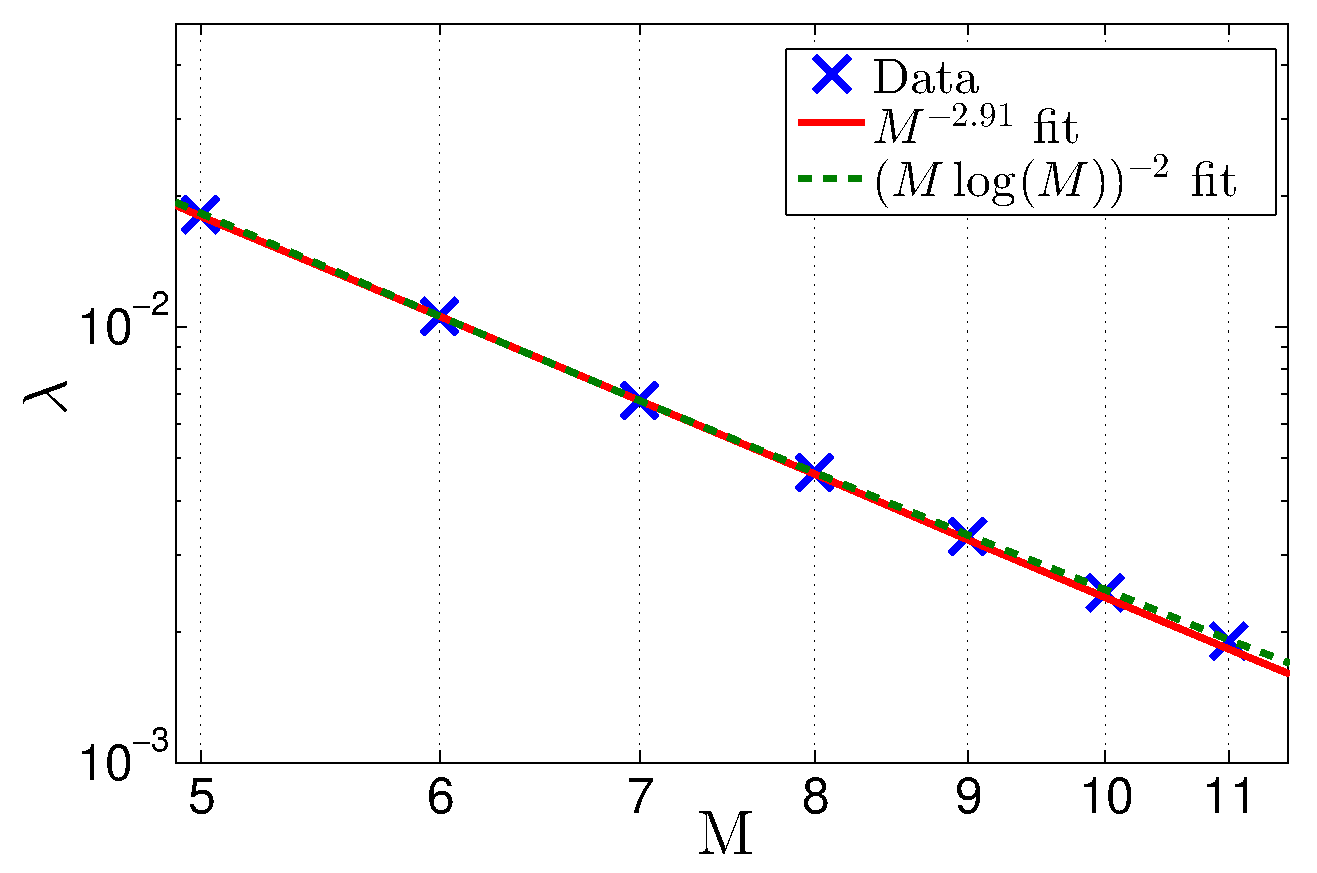
\includegraphics[width=1.0\linewidth]{semi_infinite_full_optimal.pdf}
\centering
\caption{(color online) $\lambda$ is the minimum of Eq. \eqref{eq:minimize} for given $M$. As we increase $M$, the commutator with Hamiltonian decreases
and thus the local operator relaxes slowly. The decreasing form can be well-fitted by both a power-law and $1/(M\log(M))^2$. }
\label{fig:full_optimal}
\end{figure}

Figure \ref{fig:full_optimal} plots $\lambda$, defined to be the minimum value of the commutator with the Hamiltonian,as a function of $M$ (Eq. \eqref{eq:minimize}).
It is clear that $\lambda$ decreases with $M$.
The data can be well-fitted by two functional forms; power-law decay with exponent $2.91$ and a logarithmic correction to $1/M^2$, which is $1/(M\log(M))^2$.
In either case,
the rate of decrease with $M$ is {\it faster} than $1/M^2$, which is the scaling of the slowest diffusive energy mode as we show now.

\begin{figure}
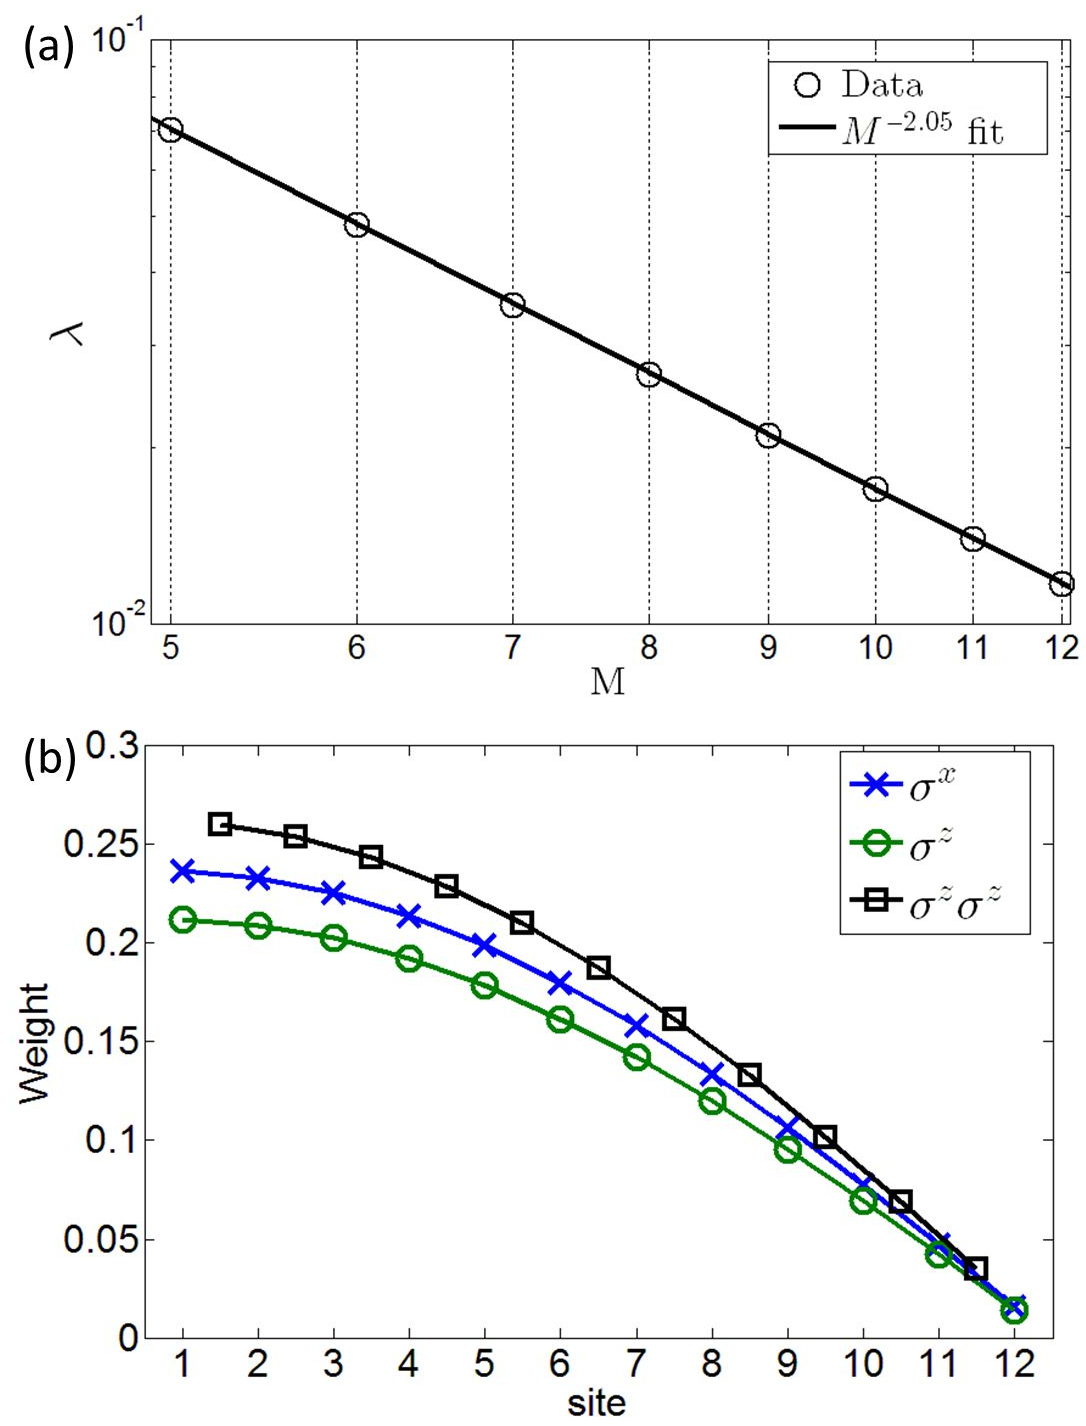
\includegraphics[width=1.00\linewidth]{Hamiltonian_only.pdf}
\centering
\caption{(color online) (a) $\lambda$ is the minimum of Eq. \eqref{eq:minimize} when only terms in Hamiltonian ($\sigma^x_i$,$\sigma^z_i$, and $\sigma^z_i\sigma^z_{i+1}$ are used. As hydrodynamics suggests, it decreases with $1/M^2$. (b) Structure of the optimal operator of $M = 12$.
We locate $\sigma^z_i \sigma^z_{i+1}$ term at site $i+1/2$. We normalize the coefficients by square norm ($\sum_\ell c_\ell^2 = 1$).
It shows a clear energy modulation with the wavelength $4(M-1)$. The relative weight of the operator is the same as relative weight of the parameters of Hamiltonian. }
\label{fig:ham_only}
\end{figure}

A slowly relaxing energy mode can be constructed by considering an energy modulation of wavelength $4M$:
\begin{align}
\hat{E}_M &= \sum_{i=1}^{M} \cos\left(\frac{(i-1)\pi}{2(M-1)}\right)(g \sigma^x_i + h\sigma^z_i)\nonumber\\
&+ \sum_{i=1}^{M-1} \cos\left(\frac{(i-1/2)\pi}{2(M-1)}\right)\sigma^z_i\sigma^z_{i+1}
\label{eq:energy_modulation}
\end{align}
Combining the continuity equation and the Heisenberg equation of motion, we have the following.
\begin{align}
\frac{d}{dt} \hat{E}_M = i[H,\hat{E}_M] = -\nabla\cdot {\bf J}_E \sim {\bf k} \cdot {\bf J}_E({\bf k}) ~,
\end{align}
where ${\bf J}_E$ is the energy current operator and the last relation is written in Fourier space, where $|{\bf k}| \sim 1/M$.
Therefore, the squared Frobenius norm of the commutator of $\hat{E}_M$ should scale as $1/M^2$.  In this case, one can explicitly compute the commutator and verify this result.

Here, we adapt a slightly more conservative approach.
We do the same numerical analysis as before but restrict the operator space within the operators in Hamiltonian.
Therefore, for a given $M$, we only use $3M - 1$ basis operators instead of $4^M-1$ without assuming any structure.
Figure \ref{fig:ham_only} (a) is the plot of $\lambda$ as a function of $M$.
As expected, we have almost perfect $1/M^2$ scaling.
Furthermore, since there are only a few basis operators, we can easily look at the details of the structure of the optimal operator.
Figure \ref{fig:ham_only} (b) depicts the structure of the optimal operator in terms of the local terms in Hamiltonian.
The structure is exactly the same as the energy modulation form of Eq. \eqref{eq:energy_modulation} with the same wavelength and relative weights.
This clearly shows that indeed the slowest mode of the conserved quantity is the modulation of the longest wavelength.


We have shown that we can numerically construct a series of local operators that relax slower (at least at early times) than
diffusive mode of the same locality. In fact, it turns out that this fully optimized local operator remains relaxing slower than diffusion for
all times.

Next, by moving into the Floquet system (for thermalization in the Floquet system, see Refs.~\onlinecite{Dalessio:2014, Lazarides:2014, Ponte:2014}),
we test whether the energy conservation is important in the slow relaxation of local operators.
As an energy non-conserving Floquet operator, we adopt the same operator used in Ref.~\onlinecite{Kim_ETH}:
\begin{align}
U_F = \exp(-i H_x \tau) \exp(-i H_z \tau) ~,
\end{align}
where $H_x$ is the $\sigma^x$ part ($\sum_i g \sigma^x_i$) and $H_z$ is the $\sigma^z$ part ($\sum_i h \sigma^z_i +\sigma^z_i \sigma^z_{i+1}$)
of the Hamiltonian. We choose $\tau = 0.8$.
Although $U_F$ does not conserve energy, it acts {\it locally} on the system.
$U_F$ is shown to thermalize a local operator at infinite temperature ensemble \cite{Kim_ETH}.
Ref.~\onlinecite{Prosen:2002} has studied a different decomposition of the same model and reports the chaotic behavior of eigenstates.

We minimize the Frobenius norm of the commutator with the Floquet operator.
Similar to Eq. \eqref{eq:minimize}, we search for the coefficients $\{ c_\ell \}$ that minimize the following:
\begin{align}\label{eq:floquet_minimize}
\frac{\mathrm{tr([\hat{A}_M,U_F][\hat{A}_M,U_F]^\dag)}}{\mathrm{tr(\hat{A}_M\hat{A}^\dag_M)}} = \sum_{\ell,k}\frac{c_\ell c_k \mathrm{tr([\hat{O}_{M,\ell},U_F][\hat{O}_{M,k},U_F]^\dag)}}{\sum_j c_j ^2 \mathrm{tr((\hat{O}_{M,j})^2)}} ~.
\end{align}
Let us first understand the physical meaning of this quantity.
As in the case of Hamiltonian system, we consider the same initial state, Eq. \eqref{eq:initial}.
It is straightforward to show that Eq. \eqref{eq:floquet_minimize} is twice of the
difference of the expectation value of $\hat{A}_M$ between the initial state and the state after one Floquet driving
[Note that time is discrete (integer multiple of $\tau$) in the Floquet system.].
\begin{align}
2\left(\langle \hat{A}_M(0) \rangle - \langle \hat{A}_M(\tau) \rangle \right) = \frac{\epsilon}{Z}\mathrm{tr([\hat{A}_M,U_F][\hat{A}_M,U_F]^\dag)} ~,
\end{align}
where $\hat{A}_M(\tau) = U_F^\dag \hat{A}_M(0) U_F$.
When $\hat{A}_M$ changes little by the initial driving, Eq. \eqref{eq:floquet_minimize} is small.
Therefore, we search for a local operator of length $M$ that retains the most of information about the initial state
after one Floquet cycle.
Figure \ref{fig:floquet} (a) is the plot of $\lambda$ (the minimum value of Eq. \ref{eq:floquet_minimize}) as a function of $M$.
Comparing to Figure \ref{fig:full_optimal} and Figure \ref{fig:ham_only},
we see that $\lambda$ decreases {\it slower} than Hamiltonian cases, which implies that the Floquet system thermalizes
the local operator {\it faster}. Since the only apparent difference between the Hamiltonian system and the Floquet system
is the existence of the energy conservation, we attribute this fast relaxation to the absence of conservation law.

\begin{figure}
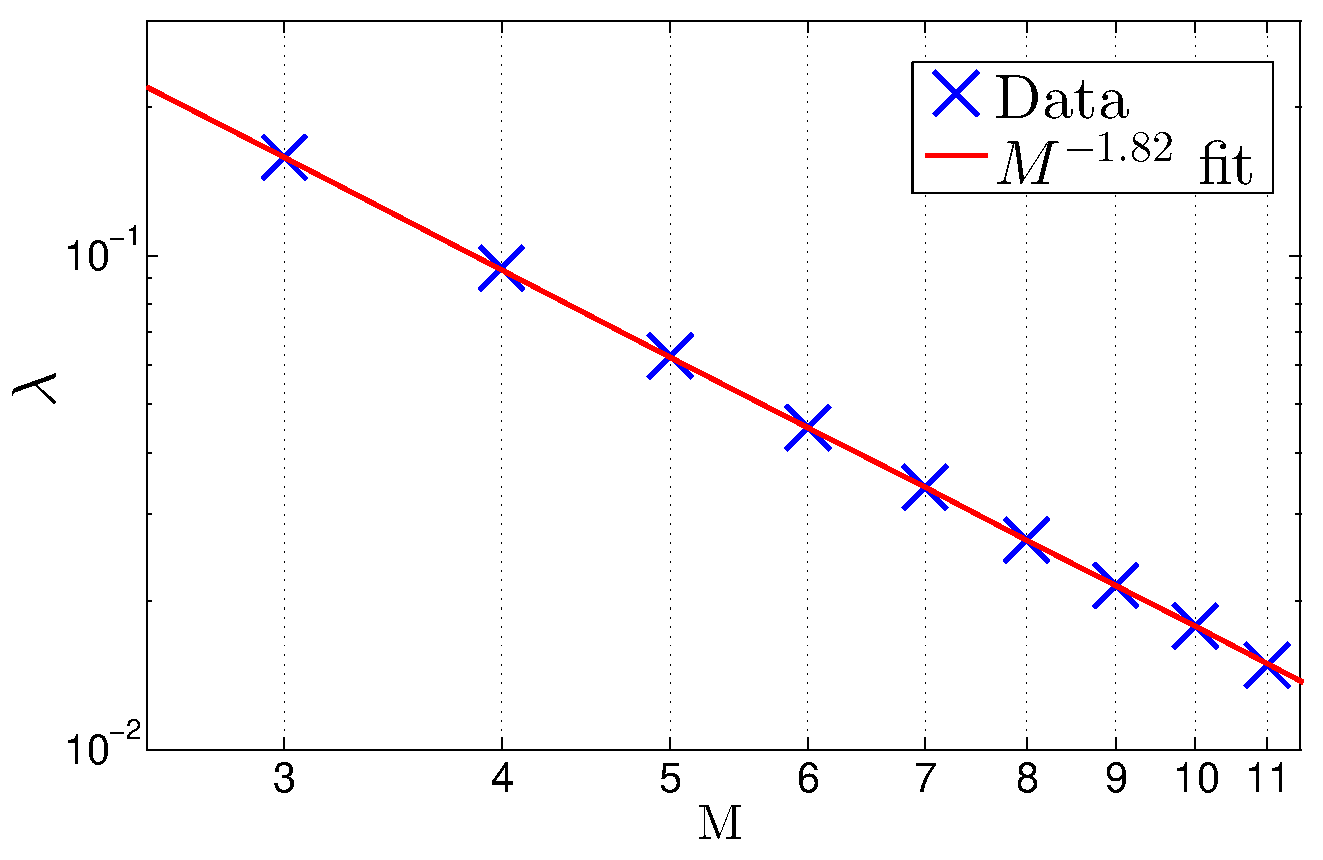
\includegraphics[width=1.0\linewidth]{semi_infinite_floquet_only.pdf}
\centering
\caption{(color online) $\lambda$ is the minimum value of Eq. \eqref{eq:floquet_minimize}. In comparison with Figure \ref{fig:full_optimal}, the Floquet system relaxes a local operator faster than the Hamiltonian system for having rather moderate decay tendency.
%(b) Decomposition of optimal operators sorted by the distance from the free edge ($M+1$'th site). Most weight is in the farthest site.}
}
\label{fig:floquet}
\end{figure}

Figure \ref{fig:floquet}, however, shows that $\hat{A}_M$ remembers more about the initial condition as the support $M$ increases.
To analyze the structure of this operator, we organize the basis operators of the optimal operator that minimize Eq. \eqref{eq:floquet_minimize}
by the distance from the free edge ($M+1$'th site) of a first non-identity operator. For example, when $M = 3$,
the basis operator $\sigma^x_1 \sigma^0_2 \sigma^x_3$ has distance 1 and $\sigma^x_1 \sigma^z_2 \sigma^0_3$ has distance 2.
We sort the basis operators by distance and sum the square of coefficients of the same distance.
Figure \ref{fig:floquet} (b) is the plot of such decomposition.
We see that more weights are placed in the sites farther from the free edge although number of such basis operators are exponentially smaller.

To determine whether this phenomenon is more generally true, we also studied a family of quantum circuits, each composed of two rounds, where in the first round, gates act on pairs of sites $...,(1,2),(3,4),...$ and on the second round gates act on pairs $...,(0,1),(2,3),(4,5),...$  We consider now an infinite, rather than semi-infinite chain.  We choose all gates in a given round to be the same, but chose them randomly.  The results are shown in Fig.~\ref{fig:lz}.  We find again that even in this random case, slow operators are present.


\begin{figure}
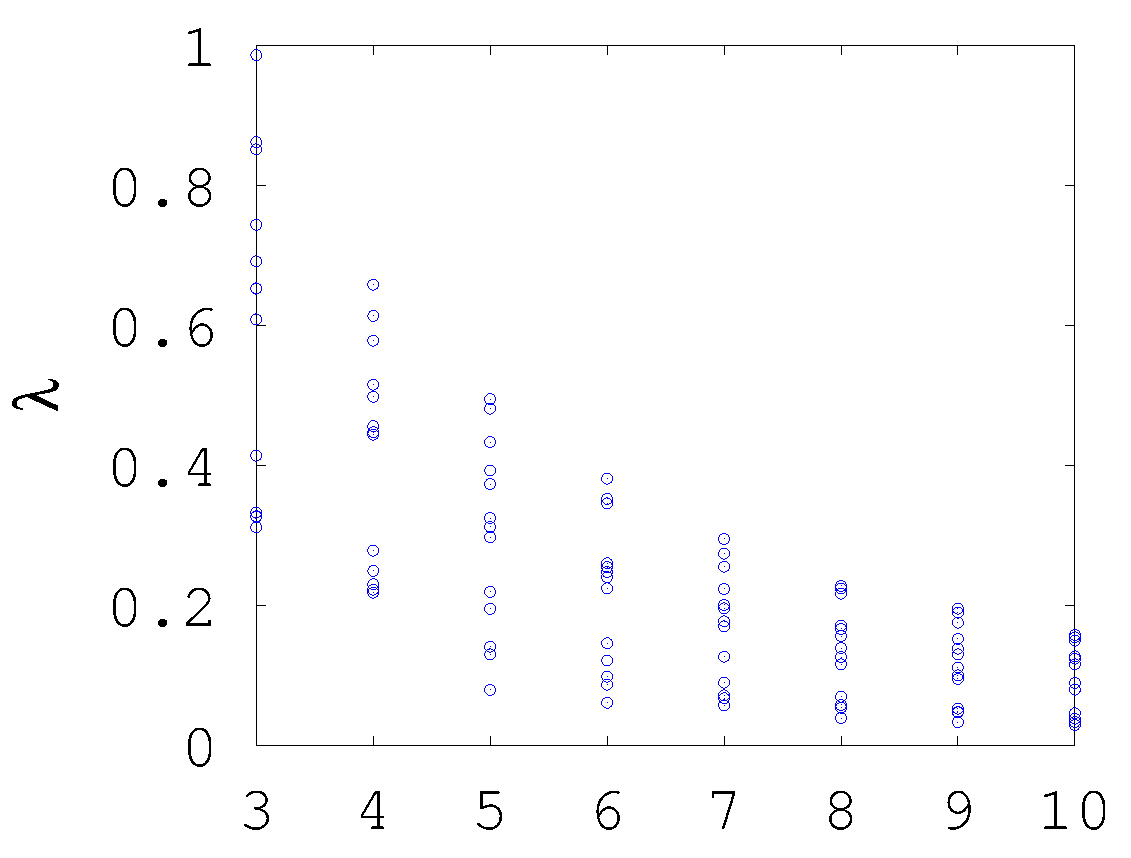
\includegraphics[width=1.0\linewidth]{circuit.pdf}
\centering
\caption{$\lambda$ as a function of $M$ for a random circuit model.  $13$ realizations are shown.  In all cases, $\lambda$ decreases with $M$.}
\label{fig:lz}
\end{figure}



{\it Summary.}
We have numerically constructed a series of local operators that relaxes (and thus thermalizes) slower than
diffusive mode of energy transport of the same locality.
We have also performed the same analysis in the similar system without energy conservation,
the Floquet system and for a family of quantum circuits, again finding slowly relaxing operators.
The structure of the operators found displays some spatial modulation, with smaller coefficients for terms nears the edge.  However the operators involve complicated many-body terms (if we restrict to just the terms in the Hamiltonian, we only obtain simpler operators related to energy currents) and so their origin remains unclear.
These operators present a new class of observables; if they can be studied experimentally, they may reveal unsuspected slow relaxation.

%\section{Results}
%\subsection{Comparison with Energy Modulation}
%\subsection{Comparison with Floquet System}
%\section{Conclusion and Discussion}
%\section{Acknowledgement}

We thank Fabian Essler for stimulating discussions and Stefan K${\rm{\ddot u}}$hn for helps in numerical algorithms.
H.K. is grateful for the support and hospitality of Max-Planck-Institute f${\rm{\ddot u}}$r Quantenoptik,
where this work has begun and Korea Institute for Advanced Study, where part of this manuscript was written.


\bibliography{slow_operator_bibl}

%\begin{thebibliography}{99}
%
%\bibitem{neumann} %von Neumann's quantum ergodic theorem
%J. von Neumann, Zeitschrift f${\rm \ddot{u}}$r Physik {\bf 57}, 30 (1929).
%
%\bibitem{shnirelman} %motivation for ETH
%A. I. Shnirelman, Usp. Mat. Nauk {\bf 29}, 181 (1974).
%
%\bibitem{berry} %berry conjecture
%M. V. Berry, J. Phys. A {\bf 10}, 2083 (1977).
%
%\bibitem{polkovnikov}
%A. Polkovnikov, K. Sengupta and M. Vengalattore, Rev. Mod. Phys. 83, 863 (2011).
%
%\bibitem{yukalov}
%V.I. Yukalov, Laser Phys. Lett. 8, 485 (2011).
%
%\bibitem{deutsch} %ETH original
%J. M. Deutsch, Phys. Rev. A {\bf 43}, 2046 (1991).
%
%\bibitem{srednicki} %ETH original
%M. Srednicki, Phys. Rev. E {\bf 50}, 888 (1994).
%
%\bibitem{rdo} %ETH popular
%M. Rigol, V. Dunjko and M. Olshanii, Nature (London) {\bf 452}, 854 (2008).
%
%\bibitem{santos} %accuracy test of ETH & hard core bosons
%L. F. Santos and M. Rigol, Phys. Rev. E {\bf 82} 031130 (2010).
%
%\bibitem{kruczenski} %thermalization using Krylov method
%M. Kruczenski and S. Khlebnikov, arXiv:1312.4612v2.
%
%\bibitem{sorg} %ETH boson model
%S. Sorg, L. Vidmar, L. Pollet and F. Heidrich-Meisner, arXiv:1405.5404v1.
%
%\bibitem{beugeling} %finitie size scaling of ETH
%W. Beugeling, R. Moessner and M. Haque, Phys. Rev. E {\bf 89}, 042112 (2014).
%
%\bibitem{rs} %checking role of ETH in quantum thermalization
%M. Rigol and M. Srednicki, Phys. Rev. Lett. {\bf 108}, 110601 (2012).
%
%\bibitem{kim_ETH}
%H. Kim, T. N. Ikeda, and D. A. Huse, arXiv:1408.0535v2.
%
%\bibitem{winter} %proof of equilibration
%N. Linden, S. Popescu, A. J. Short and A. Winter, Phys. Rev. E {\bf 79}, 061103 (2009).
%
%\bibitem{ruelle}
%D. Ruelle, J. Stat. Phys. {\bf 44}, 281 (1986).
%
%\bibitem{prosen} %first exploration of dynamics of local operators in detail
%T. Prosen, J. Phys. A {\bf 35}, L737 (2002).
%
%\bibitem{banuls} %observatino of nonthermalization in the model Hamiltonian
%M. C. Ba${\rm{\tilde n}}$uls, J. I. Cirac, and M. B. Hastings, Phys. Rev. Lett. {\bf 106}, 050405 (2011).
%
%\bibitem{kim1} %parameter choice of the model
%H. Kim and D. A. Huse, Phys. Rev. Lett. {\bf 111}, 127205 (2013).
%
%\bibitem{luca} %Circular Ensemble
%L. D'Alessio and M. Rigol, arXiv:1402.5141v1.
%
%\bibitem{lazarides} %floquet 1
%A. Lazarides, A. Das and R. Moessner, arXiv:1403.2946v1.
%
%\bibitem{ponte} %floquet 2
%P. Ponte, A. Chandran, Z. Papi\'c and D. A. Abanin, arXiv:1403.6480v1.
%
%\bibitem{kim_realtime}
%H. Kim, {\it et. al.}, in preparation.
%
%\bibitem{fernando} F. G. S. L. Brandao, A Harrow, and M. Horodecki, arXiv:1208.0692.
%
%\end{thebibliography}

\section*{Supplementary Material}

\subsection{Operator Norm}
In the main text, we have used the square of the Frobenius norm to quantify the commutator with the Hamiltonian.
This quantifies the relaxation of $\hat{A}_M$ at $t = 0$,
which is not precisely what we want. Ideally, we want to find a local operator
that relaxes the slowest in the long time.
For that purpose, we need to consider the operator norm (the largest eigenvalue in magnitude).

Assuming that $\hat{A}_M$ satisfies the following:
\begin{align}
||[\hat{A}_M, H]|| \leq \chi(M),
\end{align}
where $H$ is the Hamiltonian and $||\ldots||$ means the operator norm of the argument and $\chi(M)$ is some nonnegative valued function.
Then, using the Heisenberg equation of motion, we have
\begin{align}
\bigg|\bigg|\frac{d}{dt} \hat{A}_M(t)\bigg|\bigg| &= \bigg|\bigg| e^{-i H t} \left(\frac{d}{dt} \hat{A}_M (t)\right) e^{i H t} \bigg|\bigg| \nonumber\\
&= ||[\hat{A}_M(t = 0), H]|| \leq \chi(M) \\
||\hat{A}_M(t) - \hat{A}_M(0)|| &= \bigg|\bigg|\int_0^t \left(\frac{d}{d\tau} \hat{A}_M(\tau)\right)d\tau \bigg|\bigg| \nonumber\\
&\leq \int^t_0 \big|\big|\frac{d}{d\tau} \hat{A}_M(\tau)\big|\big|d\tau \leq \chi(M) t ~,
\end{align}
where we have used the fact that $e^{-iHt}$ is a norm-preserving unitary operator.
This inequality bounds the distance of an operator evolving under Hamiltonian dynamics
from its initial configuration. Next, we consider an initial state $\rho$ such that
\begin{align}
|\langle \hat{A}_M \rangle_0 - \langle \hat{A}_M \rangle_\beta| = \gamma(M) ~,
\end{align}
where $\langle \ldots \rangle_0$ is expectation value of initial condition and $\langle \ldots \rangle_\beta$
is thermal expectation value and $\gamma(M)$ is some nonnegative valued function.
Now we can estimate the distance between thermal expectation value and expectation value at time $t$ (for $t \leq \gamma(M)/\chi(M)$):
\begin{align}
&|\langle \hat{A}_M \rangle_t - \langle \hat{A}_M \rangle_\beta| \nonumber\\
&\geq ||\langle \hat{A}_M\rangle_0 - \langle \hat{A}_M\rangle_\beta | -|\langle \hat{A}_M\rangle_t - \langle \hat{A}_M\rangle_0 || \nonumber\\
&\geq \gamma(M) - t \chi(M)
\end{align}
where $\langle \ldots \rangle_t$ is expectation value at time $t$.
Therefore, if we have a sequence of $M$-body operators $\{ \hat{A}_M \}$
whose operator norm of the commutator with Hamiltonian decays fast with $M$
\footnote{When $M\rightarrow\infty$, $\hat{A}_M$ can be a projection onto an eigenstate of Hamiltonian so it commutes with $H$.},
and an initial state which does not allow fast decrease of $\gamma(M)$,
the time scale of thermalization of $\hat{A}_M$ is
\begin{align}
\tau_M \sim \frac{\gamma(M)}{\chi(M)} ~.
\end{align}
In particular, if $\chi(M) \sim \exp(-\alpha M)$ with some positive $\alpha$ and $\gamma(M)$ does not decrease exponentially,
thermalization may take exponentially long with $M$ as opposed to polynomially long in case of diffusion.

However, optimizing the operator norm is numerically very challenging.
Therefore, we used the Frobenius norm, which is much simpler to compute, to construct slowly relaxing local operators
and we still found nontrivial results.

\subsection{Results of another set of parameters in Hamiltonian}
\begin{figure}
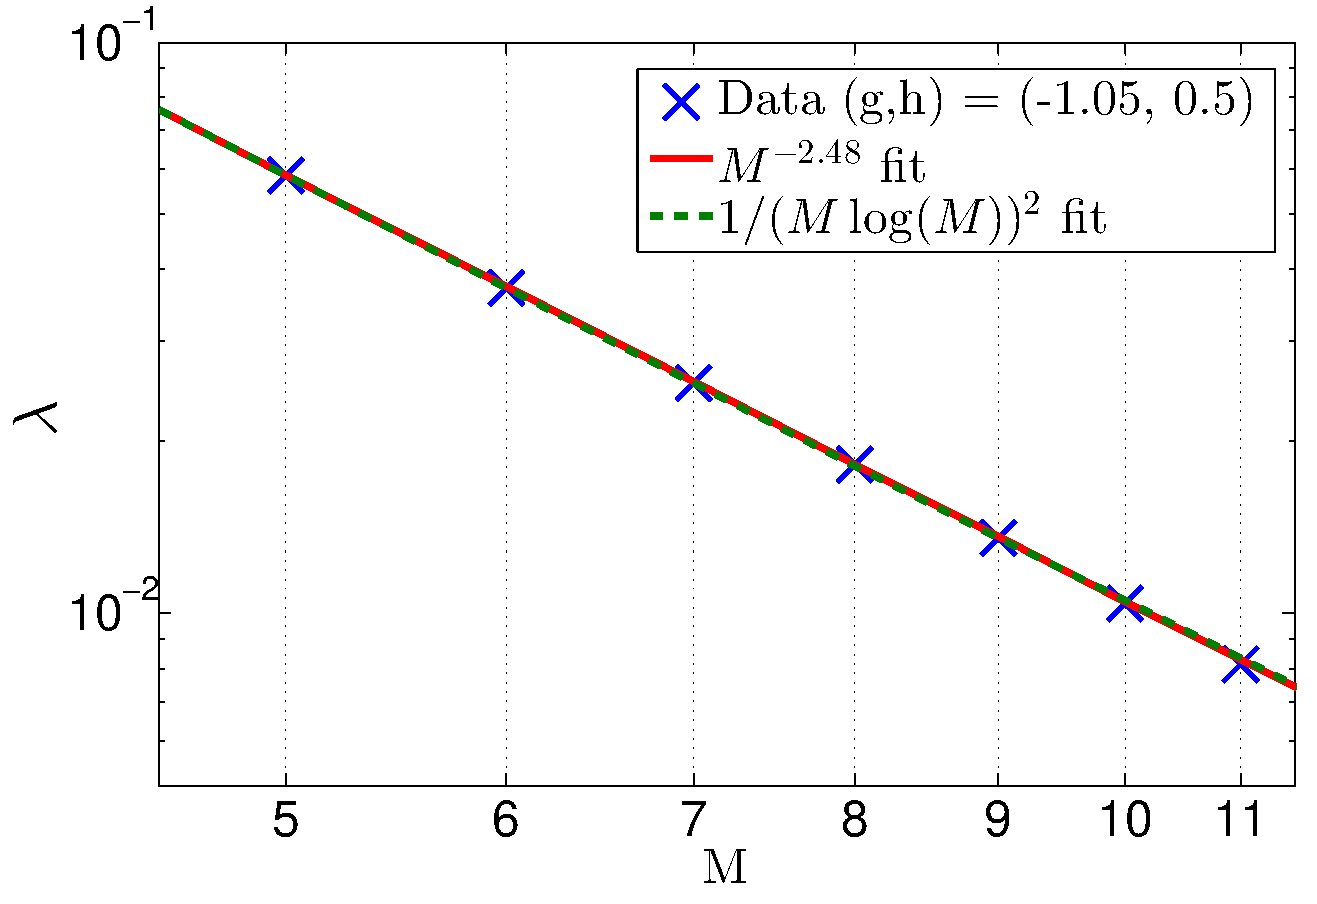
\includegraphics[width=1.0\linewidth]{semi_infinite_full_optimal_other_parameter.pdf}
\centering
\caption{(color online) $\lambda$ is the minimum value of the Frobenius norm of the commutator with Hamiltonian for given $M$.
Here we choose the parameters to be $(g,h) = (-1.05, 0.5)$. $\lambda$ still decreases faster than $1/M^2$. }
\label{fig:full_optimal_other}
\end{figure}
In this section, we show that the main results in the main body do not depend on the parameter choice.
We choose another set of parameters $(g,h) = (-1.05, 0.5)$, which is the parameter choice of Ref.~\onlinecite{Banuls:2011}.

Figure \ref{fig:full_optimal_other} is the minimum value of Eq. \eqref{eq:minimize} with the other parameter choice.
We can see that it decays faster than $1/M^2$. As is the case of the parameter choice in the main body,
the data can be well-fitted by two methods; a power-law and a logarithmic correction to $1/M^2$.
Since the power-law exponent could depend on the parameter choice, we do not attempt to draw a strong conclusion from this data
except that $\lambda(M)$ (minimum of the Frobenius norm of the commutator with Hamiltonian) decreases faster than $1/M^2$,
which is the scaling of the diffusive energy mode.

\begin{figure}
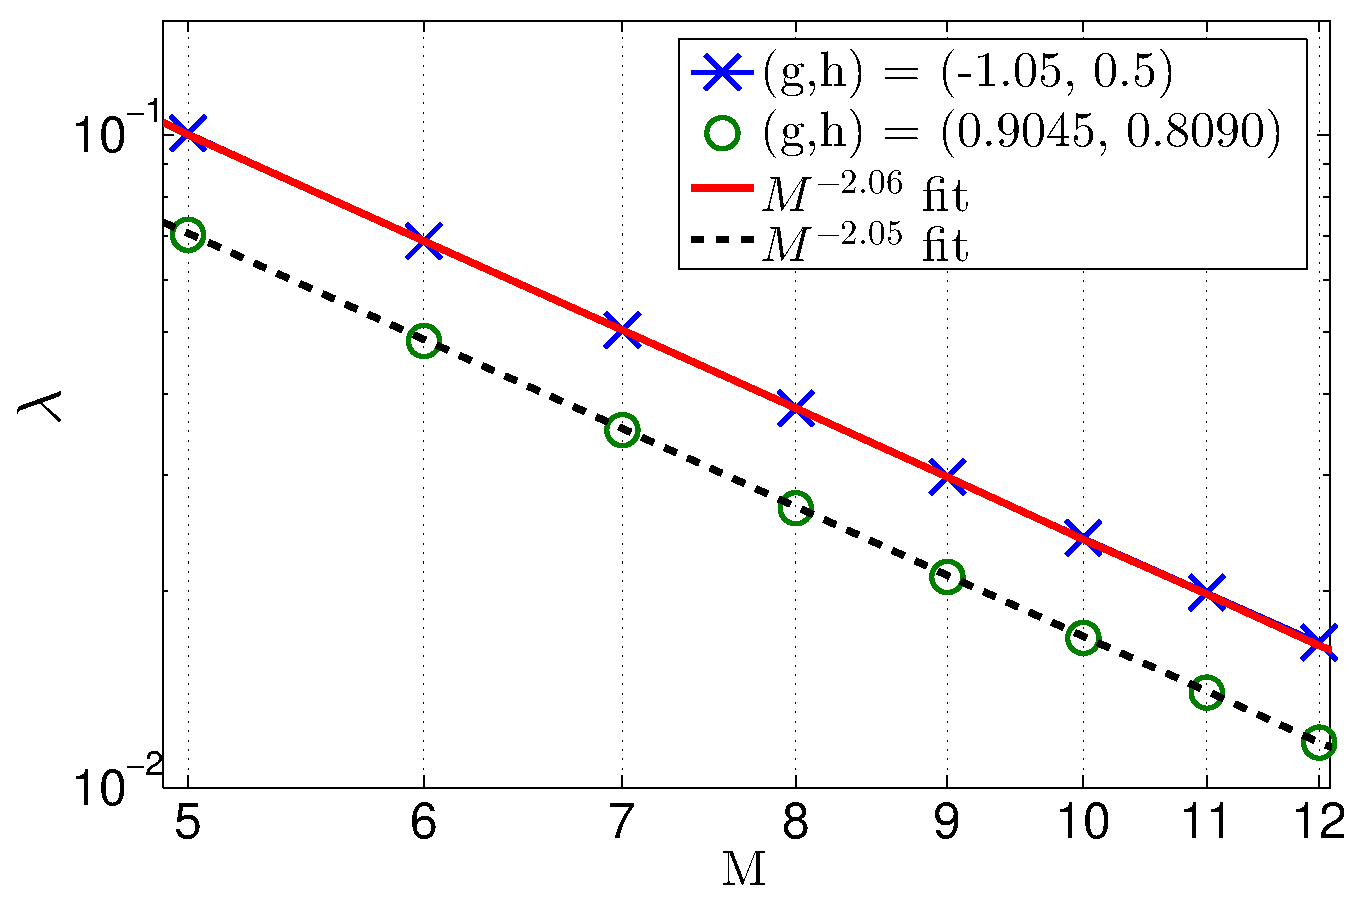
\includegraphics[width=1.0\linewidth]{X_Z_ZZ_only_two_parameters.pdf}
\centering
\caption{(color online) $\lambda$ is the minimum value of Eq. \eqref{eq:minimize} when only terms in Hamiltonian are used. We see that $1/M^2$ scaling, which comes from the energy modulation holds for both parameter choices. }
\label{fig:Ham_only_two_parameters}
\end{figure}
Figure \ref{fig:Ham_only_two_parameters} is the plot of the minimum value of Eq. \eqref{eq:minimize} when only terms in Hamiltonian are allowed
for two sets of parameters. Unlike the case where all operators are used,
the decay scaling remains the same as $1/M^2$ as expected from the hydrodynamics.
Therefore, we again explicitly demonstrate that the longest wavelength energy modulation is the slowest mode of a conserved quantity.



Figure \ref{fig:floquet_two_parameters} shows the minimum value of the commutator with the Floquet operator in the Flobenius norm.
We see that the $M$ scaling does not depend on the parameter choice, unlike Hamiltonian system.
This may hint us that the mechanism of slowing down the relaxation in the Floquet system, where no local conservation law is present,
could be universal.

\begin{figure}
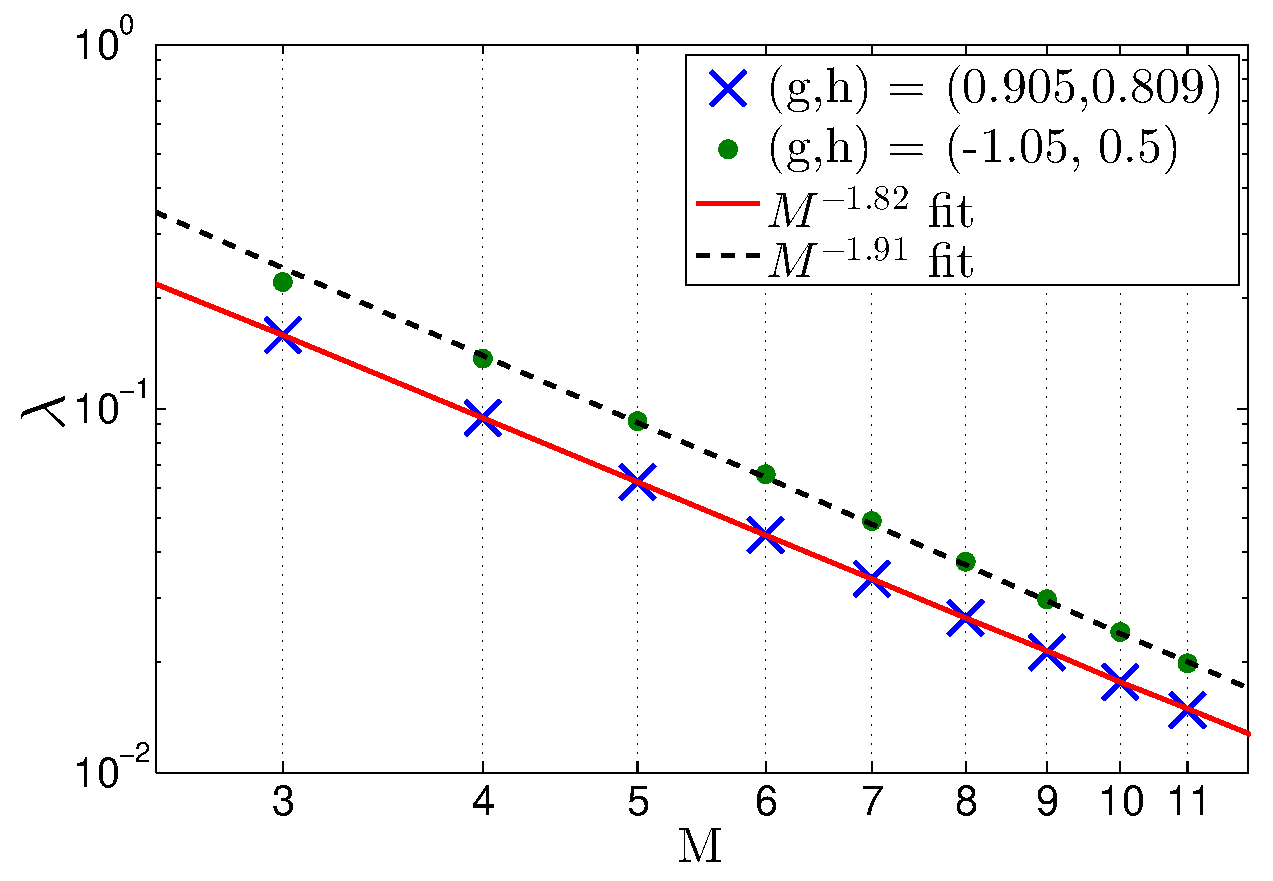
\includegraphics[width=1.0\linewidth]{semi_infinite_floquet_two_parameters_extended.pdf}
\centering
\caption{(color online) }
\label{fig:floquet_two_parameters}
\end{figure}





\end{document} 
